\Chapter{Bases sur la physique des plasmas magnétisés}
\label{Introduction}
\begin{refsection}

\section{Fondamentaux et échelles caractéristiques}
\subsection{Les plasmas}
L'état de plasma est souvent considéré un peu équivoquement comme
le quatrième état de la matière. Quand elle est portée à des températures
de plus en plus élevées, celle-ci passe en effet successivement par les états
solide, liquide, gazeux, puis plasma (voir figure~\ref{1-plasma}).

En réalité,
une définition plus correcte serait celle d'un état gazeux partiellement ou
totalement ionisé, c'est à dire possédant une population d'électrons et
d'ions, possiblement de différentes espèces. Ces populations de charges
libres, qui sont sensibles aux forces électromagnétiques, permettent alors le transport de
courant et influencent fortement le comportement global du plasma, provoquant
l'apparition de phénomènes collectifs et souvent non-linéaires.

\begin{figure}[htbp]
\centering
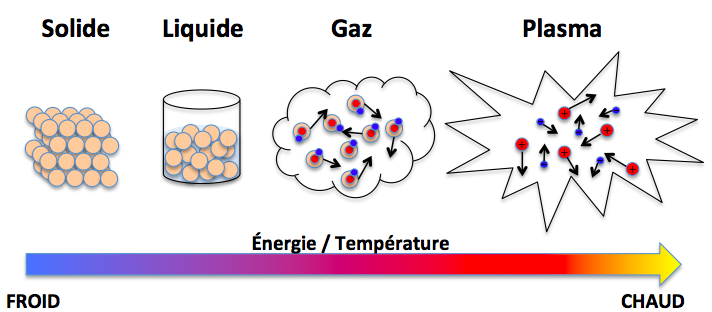
\includegraphics[width=0.8\textwidth]{figures/1-plasma.png}{\caption{Évolution
des états de la matière en fonction de la température.}\label{1-plasma}}
\end{figure}

Historiquement, nous avons pris conscience de l'existence des plasmas à travers
les phénomènes de flammes, d'éclairs et d'aurores boréales, mais à des
conditions de pression et de température différentes de celles de l'atmosphère
terrestre, ils sont omniprésents : dans l'espace intergalactique et
intersidéral, dans le vent solaire et les étoiles, 99\% de la matière connue
est sous cette forme.

De nos jours, l'homme créé artificiellement des plasmas pour de nombreuses
applications : les dispositifs d'affichage et d'éclairage, le traitement et la
gravure de matériaux, la propulsion spatiale ou encore la fusion
thermonucléaire contrôlée, sont autant d'exemples pour lesquels la maîtrise des
plasmas est essentielle.

Le comportement des plasmas est décrit par la théorie de la physique des
plasmas qui intègre les connaissances de nombreux domaines, tels que la
physique statistique, l'électromagnétisme, ou encore la dynamique des fluides.
Le premier chapitre rappelle quelques bases théoriques sur cette physique,
nécessaires à la compréhension des travaux présentés et à l'autosuffisance du manuscrit.

\subsection{Les paramètres plasmas}
Les plasmas se présentent donc comme des gaz dont le comportement est influencé
de manière non négligeable par une population de charges libres.
La population électronique permet de définir deux paramètres principaux :

\begin{itemize}
  \item la densité $n_e$ mesurant le nombre
  de particules par élément de volume ;
  \item la température électronique $T_e$ mesurée en unité
  d'énergie\footnote{Il existe une deuxième façon de noter la
  température électronique, que l'on peut retrouver dans beaucoup d'ouvrages
  et de papiers de la communauté plasmas froids, issue du postulat suivant : si
  $T_e$ en [K] $\rightarrow k_BT_e$ en [J] donne par analogie si
  $T_e$ en [eV] $\rightarrow eT_e$ en [J]. La constante $e$ étant définie
  en [C], $T_e$ mesure alors une tension et 1 eV $\sim$ 1 V.}, représentative de
  l'énergie cinétique moyenne non dirigée des électrons (aussi appelée agitation
  thermique).
\end{itemize}

\begin{equation}
\label{1-VThermique}
	T_{e}=m_{e} v_{{T}_{e}}\puissance{2}
\end{equation}

où $m_{e}$ est la masse de l'électron, et $e$ la charge élémentaire. Pour un
électron possédant une énergie de 1 eV, la vitesse thermique
$v_{{T}_{e}}$ est de l'ordre de 4.10$^5$~m/s. À même énergie, du fait de la
différence de masse, cette vitesse est bien inférieure pour les ions (quand les
concepts de température et de vitesse thermique ont un sens) et vaut par exemple
10$^3 $~m/s dans le cas de H$^+$ :

\begin{equation}
	v_{{T}_{i}}\sim\left(m_{e}/m_{i}\right)^{\text{\textonehalf}}
	v_{{T}_{e}}
\end{equation}

La figure (\ref{zoologie}) représente une classification des plasmas
en fonction de ces deux paramètres principaux qui vont influer sur la dynamique du
transport des particules et du courant.

\begin{figure}[htbp]
\centering
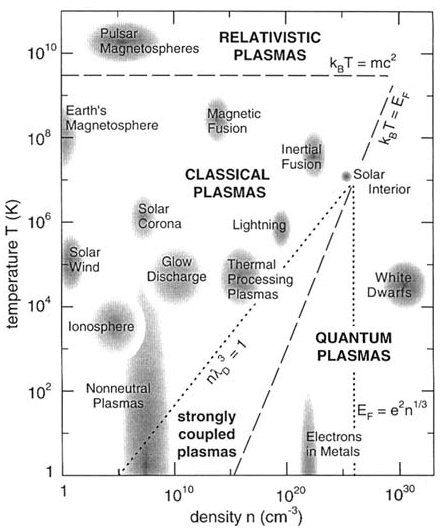
\includegraphics[height=80mm,width=64mm]{figures/1-zoologie.png}{\caption{Classification
de différents plasmas en fonction de $n_e$ et $T_e$ issue du livre du National
Research Council \parencite{NRC}}\label{zoologie}}
\end{figure}

L'ionisation du gaz suit l'évolution de la température
électronique $T_{e}$ ;
dans les plasmas, le degré d'ionisation $\alpha$ est donné par le rapport
entre la densité électronique $n_{e}$ et la densité de gaz neutre
$n_{g}$ :

\begin{equation}
\alpha=\frac{n_{e}}{n_{e}+n_{g}}
\end{equation}

Cette fraction va définir l'importance de l'interaction entre les particules
neutres et les particules chargées. Cependant, même à très faible $\alpha$,
l'apparition d'une population de porteurs de charge va modifier considérablement 
les caractéristiques et la dynamique du plasma.
Densité et température électroniques permettent de définir le paramètre de couplage $\Xi$ :

\begin{equation}
\label{1-paramPlasma}
\Xi=\frac{<E_\text{p}>}{<E_\text{c}>}=\frac{e\puissance{2}
n_{e}\puissance{1/3}}{\varepsilon\indice{0} T_{e}}
\end{equation}

Le paramètre de couplage représente le ratio entre l'énergie thermique des
électrons et leur énergie potentielle électrostatique coulombienne, i.e.
l'agitation thermique désordonnée contre les forces d'interactions
coulombiennes structurantes.

Les plasmas classiques (ou cinétiques) sont caractérisés par
$\Xi\ll$ 1. Ils ont une population d'électrons assez espacée et/ou une
température suffisamment élevée. La théorie présentée dans cette thèse ne
concerne que ce type de plasma, i.e. :

\begin{itemize}
  \item les plasmas naturels peu denses tels que l'espace interstellaire,
  le vent solaire, la magnétosphère, et l'ionosphère
  \item les plasmas naturels denses tels que les éclairs et les étoiles
  \item les plasmas industriels, de laboratoire, et thermonucléaires
\end{itemize}

Le plasma a naturellement tendance à suivre les champs extérieurs tout en
restant fortement couplé. Dans un premier temps, les ions et les électrons
se regroupent et vont ensemble afin de maintenir un équilibre électrostatique ;
une quasineutralité s'établit au sein du plasma. Dans un deuxième temps,
le transport réagit aux champs appliqués. L'évolution quasineutre du plasma,
plus lente, tend alors à former un équilibre entre le déplacement des particules
et la valeur locale et instantanée des champs de force extérieurs.

\subsection{Quasineutralité et phénomène d'écrantage}
La dynamique d'un plasma résulte du couplage entre le mouvement des
particules chargées et les forces électromagnétiques présentes ou qui se
forment dans le système :

\begin{equation}
\frac{\text{d} \mathbf
v_\alpha}{\text{dt}}=\frac{q_\alpha}{m_\alpha}(\mathbf E+ \mathbf
v_\alpha\times\mathbf B)
\end{equation}

l'indice $\alpha$ dénotant le type de la particule chargée, $m_\alpha$
et $q_\alpha$ sa masse et sa charge, $\mathbf v_\alpha$ sa vitesse. Le champ
électromagnétique $(\mathbf E,\mathbf B)$ peut généralement se décomposer en
deux parties :
un champ extérieur, souvent imposé par l'homme pour
contrôler le plasma, et un champ auto-cohérent, créé par le plasma lui même en
réponse à la séparation et au déplacement des charges (équations de
Maxwell-Gauss et Maxwell-Ampère).
Le champ magnétique généré par les courants du plasma étant
généralement assez faible, il est commun de
ne considérer que le champ appliqué pour étudier le comportement du
plasma\footnote{Pour le champ électrique, la situation peut varier suivant le
type d'expérimentation : dans les sources de plasma froid, le champ extérieur
peut être utilisé pour contrôler la décharge ; dans les tokamaks, c’est
principalement le plasma qui l’auto-génère.}.

L'un des processus les plus rapides que l'on peut trouver dans un plasma est lié à
l'équilibre microscopique électrostatique qui s'opère
entre l'agitation thermique et l'interaction coulombienne des particules. Les
ions et les électrons issus de l'ionisation se réorganisent spontanément pour former un ensemble électriquement neutre.
Tout écart à la neutralité, définie par une densité d'ions égale à celle des
électrons, entraîne l'apparition d'un fort champ électrique de rappel à
l'équilibre suivant la loi de Maxwell-Gauss :

\begin{align}
\label{1-Max-Poisson}
\nabla\cdot\mathbf{E}=\frac{q_in_{i}+q_en_{e}}{\varepsilon\indice{0}}
\end{align}

où $\varepsilon\indice{0}$ est la constante diélectrique du
vide et $q_in_{i}+q_en_{e}$ la densité spatiale de charge. 
En appliquant la première loi de Newton à un électron, deux
échelles caractéristiques apparaissent : la fréquence de Langmuir, ou pulsation
plasma $\omega_{pe}$ et la longueur de Debye $\lambda_D$, toutes deux reliées
par l'intermédiaire de la vitesse thermique électronique \eqrefp{1-VThermique}:

\begin{equation}
\underbrace{\sqrt{\frac{n_e
e\puissance{2}}{\varepsilon\indice{0}
m_{e}}}}_{\omega_{pe}}\cdot\underbrace{\sqrt{\frac{\varepsilon\indice{0}
T_{e}^{{\phantom{1}}}}{n_e e\puissance{2}}}}_{\lambda_D}
=\underbrace{\sqrt{\frac{T_{e}^{{\phantom{1}}}}{m_{e}}}}_{v_{{T}_{e}}}
\end{equation}

La pulsation plasma $\omega_{pe}$ correspond à la fréquence typique
d'oscillation des électrons en réponse à une petite séparation de charge. En
conséquence, des processus plus lents que cette fréquence ne voient
apparaître aucun écart à la neutralité.

La longueur de Debye $\lambda_\text{D}$, quant à elle, permet de définir le
phénomène d'écrantage :
C'est une longueur au-delà de laquelle le champ électrique créé par une particule est \emph{écranté} par 
un nuage de particules de charge opposée. Dans un plasma, chaque particule est
écrantée et participe à l'écrantage des autres ; le nombre de particules présentes
dans la sphère de Debye, de rayon $\lambda_\text{D}$, définit alors un paramètre
adimensionné, $N_D=4\pi/3\,n_e\lambda_D^3$ semblable au paramètre de couplage
$\Xi$ \eqrefp{1-paramPlasma}. Un grand nombre de particules dans la sphère de Debye
$N_D\gg1$ caractérise un plasma idéal, i.e. où le
phénomène d'écrantage électrique est dominant.

Au delà de ces échelles, le plasma est dans un état de \emph{quasineutralité}
\footnote{La quasineutralité n'est pas la seule conséquence de ce phénomène de
réorganisation de charges : lors de l'application d'un champ électrique ou magnétique, celui-ci est rapidement
écranté par le plasma, les particules s'agencent afin de créer un champ
opposé.}, i.e. où :

\begin{equation}
n_e=n_i
\label{quasineutralité}
\end{equation}

L'interaction coulombienne d'une particule chargée avec l'ensemble des autres particules peut alors
se réduire à son interaction avec un potentiel électrique local $\Phi$,
résultant de la somme des potentiels microscopiques individuels.

Le système évolue ensuite sur cet équilibre par le biais de
\emph{phénomènes de transport} résultants de l'influence
globale des champs électromagnétiques et de la tendance à
l'homogénéisation du plasma.
Ces processus interviennent sur des échelles relativement
lentes et relativement grandes devant $\omega_{p}$ et $\lambda_\text{D}$ :

\begin{equation}
\omega\ll \omega_{p}
\;\;\;\;\text{et}\;\;\;\;l\gg\lambda_\text{D}
\end{equation}

$\omega$ étant une fréquence caractéristique et $l$ une longueur typique
du processus de transport considéré. Dans les phénomènes de transport
collisionnel, on parle de diffusion/convection de particules, de viscosité
(diffusion de quantité de mouvement), de conductivité (transport de charges) ou
encore de conductivité thermique (transport de chaleur).


\subsection{Collisions}
\label{1-Collisions}
En plus de l'interaction coulombienne globale de l'ensemble des espèces chargées, 
les particules, prises deux à deux, peuvent interagir binairement. 
Ces interactions directes entre particules donnent lieu à des transferts
d'impulsion, d'énergie ou encore à des réactions plus complexes telles que
l'ionisation, l'excitation et la recombinaison ; elles sont regroupées
sous le terme général de collisions et sont caractérisées à l'échelle
microscopique par des sections efficaces de collision. La fréquence de
collision $\nu_{\alpha \beta}$, qui donne pour une réaction la probabilité
d'interaction par unité de temps d'une particule de l'espèce $\alpha$ sur une
population cible $\beta$, est définie par :

\begin{equation}
\label{1-collisionfreq}
	\nu_{\alpha
	\beta}(v_r)=n_\beta\sigma_{\alpha
	\beta}(v_r)\,v_r
\end{equation}

où $n_\beta$ est la densité de l'espèce cible, $\sigma_{\alpha \beta}$ est la
section efficace de collision et $v_r=|v_\beta-v_\alpha|$ le module de
la vitesse relative entre la particule incidente et la cible. 
Le cas des collisions entre les particules chargées et le gaz peut souvent se
simplifier davantage en négligeant la vitesse du gaz (quand celui-ci est au repos et forme
un fond diffus pour le plasma), de sorte que $v_r=v_\alpha$.

La relation \eqref{1-collisionfreq}
concerne une particule de vitesse $v_\alpha$ ; pour tenir compte de l'ensemble des particules
de l'espèce et obtenir un coefficient macroscopique, on prend la moyenne de
cette fréquence sur la distribution en vitesse :

\begin{equation}
\label{1-collisionfreqMacro}
	\left<\nu_{\alpha
	\beta}\right>_v=n_\beta\left<\sigma_{\alpha
	\beta}(v_r)\,v_r\right>_v=n_\beta k_{\alpha
	\beta}
\end{equation}

$k_{\alpha\beta}=\left<\sigma_{\alpha\beta}
v_r\right>$ définit alors un taux de collision/réaction macroscopique, qui se
mesure en m$^{3}$/s, associé à l'interaction. Pour les électrons, ce taux de
collision se calcule généralement en
supposant une distribution maxwellienne (et donc fonction de $T_e$) et en
négligeant la température du gaz, soit en l'estimant à travers une approximation
de champ local\footnote{En considérant une population d'électrons dans une petite zone de plasma en interaction avec le gaz et
dans un champ électrique $\mathbf E$ homogène, un équilibre se forme entre
l'énergie gagnée par l'accélération dans $\mathbf E$ et celle perdue dans les
collisions. C'est ce qu'on appelle un équilibre de champ local.} : le taux
s'exprime alors en fonction du ratio entre la valeur locale du champ
électrique et de la densité de neutres $\mathbf E/n_g$.

Pour les ions la fonction de distribution est plus difficile à déterminer ; on a
alors recours à des expériences spéciales dites de
"swarm"~\parencite{Ellis,Phelps} pour mesurer $\nu$ indirectement à partir de
modèles de Dérive-Diffusion
(voir~\S~\ref{ApproximationsEqMvt}-\ref{1-transportAmbipolaire}).

\subsubsection{Collisions élastiques et inélastiques}

Lors de collisions
\emph{élastiques}\footnote{Les collisions sont dites élastiques car elles
donnent lieu à des transferts d'impulsion et d'énergie sans changer la nature
des particules à l'issue de la collision.}, les particules échangent de
l'énergie en fonction de leur ratio de masse. Dans les collision entre les
électrons et les espèces plus lourdes, les premiers sont diffusés de façon
aléatoire et perdent donc de la quantité de mouvement au profit d'une isotropisation globale
des vitesses électroniques.
Au contraire, dans les plasmas froids, les ions ont tendance à céder une grande partie de leur énergie aux
neutres omniprésents et leur température reste voisine de celle du gaz. 

Dans le cas des plasmas totalement ionisés, seules les collisions coulombiennes 
(interactions binaires entre particules chargées dues à la force de Coulomb)
sont présentes. 
La fréquence de collision macroscopique $\left<\nu_{ei}\right>_v$ caractérise alors la
fréquence de transfert de quantité de mouvement entre les électrons et les ions
dans les collisions coulombiennes :

\begin{equation}
	\left<\nu_{ei}\right>_v\sim\frac{4\sqrt{2\pi}e\puissance{4} n_{e} \ln\Lambda
	}{3(4\pi\varepsilon\indice{0})\puissance{2}m_{e}\puissance{1/2}T_{e}\puissance{3/2}}
\end{equation}

avec $\ln \Lambda$ le logarithme de Coulomb,
$\Lambda=\lambda_\text{D}(e\puissance{2}/4\pi\varepsilon\indice{0}
T_{e})\puissance{-1}$ étant le ratio entre la longueur de Debye et une
distance minimale d'approche.
Contrairement aux collisions avec le gaz, les
collisions coulombiennes résultent en une redistribution de la quantité de
mouvement et de l'énergie au sein du plasma.

Les collisions avec le gaz peuvent aussi entraîner des réactions plus complexes
au cours desquelles les particules changent de nature ou d'état (ionisation,
attachement électronique, excitation\ldots).
Ces collisions sont dites \emph{inélastiques} en opposition aux collisions
élastiques. Parmi ces réactions, l'ionisation est le processus le plus
important car il contraint le bilan de particules et contrôle donc l'existence
du plasma. L'association de fréquences de collisions à chaque type de réaction
(eg. $\nu^\text{iz}$ pour l'ionisation), là aussi en fonction de sections
efficaces, permet un ordering sur l'importance de ces processus dans l'évolution
du plasma.

\subsubsection{Libre parcours moyen}

En plus d'une fréquence, on associe souvent une longueur caractéristique
à l'occurrence d'une collision. Le libre parcours moyen $\lambda_\alpha$
représente alors la distance que peut parcourir une particule à une vitesse
$v_\alpha$ avant de subir une interaction avec le système qui l'entoure :

\begin{equation}
	\lambda_\alpha=\frac{\left<v_\alpha\right>}{\left<\nu_\alpha\right>}
	=\frac{\left<v_\alpha\right>}{n_g\left<\sigma_\alpha v_\alpha\right>}
\end{equation} 

La collisionnalité d'une espèce est enfin
définie par le ratio entre son libre parcours moyen $\lambda_\alpha$ et la
taille $L$ du plasma. Quand le libre parcours moyen est petit devant la
taille du plasma $\lambda_\alpha/L\ll 1$
les particules ont le temps de faire de nombreuses collisions avant de
traverser entièrement le système. Dans les plasmas basse-pression, où la
fréquence d'ionisation est souvent plus élevée que la fréquence de collision
ions-neutres, la longueur caractéristique du transport ionique est alors reliée
à une certaine longueur d'ionisation $\lambda_\text{iz}$.

\subsection{Plasma et champ magnétique} 
\label{1-plasma-champMag}
Un plasma magnétisé est un plasma dans lequel le champ magnétique externe
$\mathbf{B}$ est suffisamment important pour modifier de manière
non-négligeable le transport des particules. Les plasmas magnétisés sont fortement
anisotropes, réagissant différemment aux forces parallèlement et
perpendiculairement au champ magnétique.

Dans un champ magnétique uniforme, le
mouvement d'une particule chargée soumise à la force de Lorentz peut se décrire
par trois composantes (cf. figure \ref{1-particleDrifts}) :

\begin{figure}[htbp]
\centering
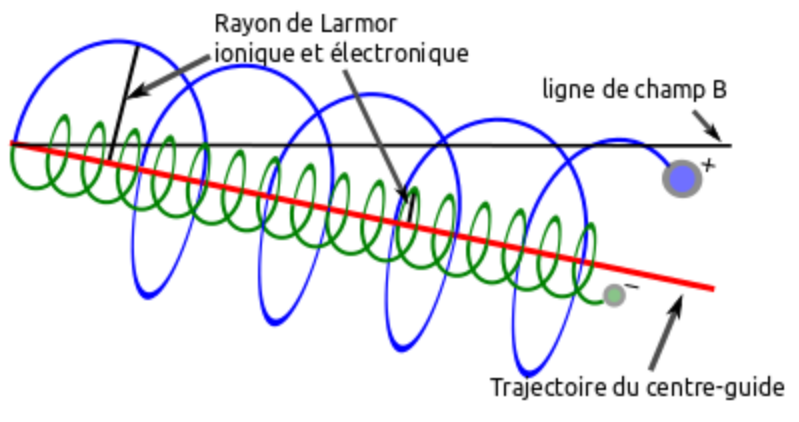
\includegraphics[width=0.7\textwidth]{figures/1-mouvementCyclotron.png}
{\caption{Mouvement cyclotronique des particules dans un champ magnétique autour
d'un centre-guide dont la trajectoire dérive lentement, dans la direction
perpendiculaire aux lignes de champ.}\label{1-particleDrifts}}
\end{figure}

\begin{itemize}
  \item Un déplacement libre le long des lignes de champ ;
  \item Un mouvement de rotation rapide de la particule
  autour d'un centre-guide dans le plan perpendiculaire à l'axe magnétique ;
  \item Une lente dérive de ce centre-guide, perpendiculairement au champ
  magnétique, qui est due aux forces extérieures.
\end{itemize}

\subsubsection{Mouvement cyclotronique}
Le mouvement de rotation autour des lignes de champ, appelé mouvement
cyclotronique, est caractérisé par la pulsation cyclotronique : 

\begin{equation}
\omega\indice{{c\alpha}}=\frac{e B}{m_\alpha}
\end{equation}

où $B$ est l'intensité du champ magnétique. Le rayon de l'orbite, appelé rayon
de Larmor $\rho_{L\alpha}$, révèle quant à lui une échelle spatiale
caractéristique du transport magnétisé.
Le rayon de Larmor se calcule en fonction de la pulsation cyclotronique et de la vitesse
$v\indice{\alpha}$ de la particule :

\begin{equation}
\rho_{L \alpha}
=\frac{v\indice{\alpha}}{\omega_{c{\alpha}}}
\end{equation}

Pour les électrons et les ions thermalisés,
la vitesse typique d'une particule est sa vitesse thermique. On peut alors noter
:

\begin{equation}
\underbrace{\frac{e B}{m_\alpha}}_{\omega_{c\alpha}}
\cdot\underbrace{\frac{\sqrt{m_\alpha T_\alpha}}{eB}}_{\rho_{L\alpha}}
=\underbrace{\sqrt{\frac{T_{\alpha}}{m_{\alpha}}}}_{v\indice{T_{\alpha}}}
\end{equation}

Quand le champ magnétique s'intensifie, les trajectoires
hélicoïdales se resserrent, limitant de plus en plus le déplacement des
particules perpendiculairement à la direction magnétique. L'influence du champ
sur le transport peut alors être mesurée par le paramètre de
magnétisation $\delta$ ; une espèce est considérée comme magnétisée à
partir du moment où son rayon de
Larmor est petit devant la longueur caractéristique $L_\perp$ du plasma,
perpendiculairement au champ magnétique :

\begin{equation}
\delta=\frac{\rho_{L\alpha}}{L_\perp}\ll 1
\end{equation}

 \subsubsection{Vitesses de dérive}

L'application d'un champ électrique conjointement à un champ magnétique
induit une troisième sorte de mouvement, appelé communément "dérive
ExB" (E-cross-B) : le phénomène de dérive se décrit comme un lent déplacement du
centre guide de la particule, perpendiculairement aux champs électrique et
magnétique. Son expression s'obtient en
prenant le produit vectoriel de l'équation de la quantité de mouvement par le
champ magnétique :

\begin{equation}
\mathbf{v}_\text{E}=\frac{\mathbf{E}\times\mathbf{B}}{B^2}
\end{equation}

Principale source de transport perpendiculaire
dans un plasma magnétisé, la vitesse de dérive électrique est indépendante de
la masse et de la charge des particules : égale pour les ions et les électrons, elle n'est donc à
l'origine d'aucun courant, ce qui la rend particulière. 

Il peut en effet apparaître d'autres vitesses de dérive. En toute généralité, 
pour chaque force $\mathbf F$ appliquée au plasma, le champ magnétique est à
l'origine d'une vitesse de dérive dans la direction perpendiculaire aux deux
forces entrant en jeu :

\begin{equation}
\mathbf{v}\indice{\text{F}}=\frac{\mathbf{F}\times\mathbf{B}}{q_\alpha B^2}
\end{equation}

Si la force $\mathbf F$ est indépendante de la charge ou
fonction de la masse de la particule, la différence entre les vitesses de dérive
des électrons et celle des ions induira un courant $\mathbf
j\indice{\text{F}}$ :

\begin{equation}
\mathbf
j\indice{\text{F}}=en(\mathbf v\indice{\text{F}{i}}-\mathbf
v\indice{\text{F}{e}})
\end{equation}.

Dans un plasma, où l'anisotropie due au champ
magnétique est souvent utilisée pour contrôler et limiter le déplacement des
particules, les vitesses de dérive sont à l'origine d'un transport
 transverse déconfinant, qui s'amplifie généralement par le développement de
 comportements non-linéaires et turbulents.
 
 \subsubsection{Paramètre de Hall}
 Dans un plasma le paramètre de Hall, $h_\alpha$, mesure l'importance du
 transport magnétisé par rapport au transport collisionnel. Il est définit par
 le ratio entre la fréquence cyclotronique $\omega_{c\alpha}$ et la fréquence
 de collision $\nu_\alpha$ :
 
 \begin{equation}
 h_\alpha=\frac{\omega_{c\alpha}}{\nu_\alpha}=\frac{eB}{m_\alpha\nu_\alpha}
 \end{equation}
 
 Le paramètre de Hall électronique peut se retrouver en mesurant l'angle de Hall
 $\theta_h$ qui se forme entre le courant dans le plasma et le
 champ électrique $h_e=\tan(\theta_h)$.
 L'effet Hall dans un plasma partiellement ionisé peut être bien plus important
 que son analogue dans les solides. En effet, souvent très inférieur à 1 dans
 les métaux, le paramètre de Hall électronique que l'on rencontre dans les
 sources magnétisées peut varier sur une large gamme de valeurs, typiquement :
 
  \begin{equation}
 0.1\,<\,h_e\,<\,1000
 \end{equation}
 
Dans nos conditions de sources magnétisées, le paramètre de
 Hall des ions ne dépasse que très rarement l'unité, ce qui signifie que ceux-ci
 ne sont que faiblement influencés par le champ magnétique.
 La différence de vitesse entre les ions et les électrons à travers le
 champ magnétique est à l'origine du courant de Hall : c'est ce courant qui
 donne son nom au propulseur à effet Hall.
 
\subsection{Les gaines électrostatiques}
\label{1-gaines}
Un plasma est souvent, à un moment ou à un autre, amené à entrer en contact avec
une paroi ou un quelconque obstacle matériel. L'interaction entre
les deux milieux conditionne alors l'existence du plasma et influence
fortement son comportement. Une paroi agit en effet comme un parfait
puit de charges et d'énergie pour le plasma, les ions et les
électrons se recombinant facilement à sa surface. Ceci étant, un plasma ne peut se maintenir
que si le nombre de particules créées dans son volume est suffisant pour
contre-balancer ces pertes en surface. 

\begin{figure}[!htbp]
\centering
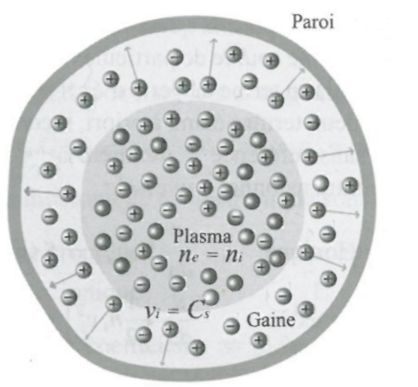
\includegraphics[width=0.45\textwidth]{figures/1-sheath.jpg}{\caption{Séparation
du plasma entre une région quasineutre et la gaine à sa
périphérie. À la frontière, il y a rupture de la quasineutralité et la vitesse
ionique, dans un plasma stationnaire, est égale à la vitesse de Bohm
$c_\text{s}$~\parencite{Rax}.}\label{1-gaine1}}
\end{figure}

De plus, les électrons, qui interceptent généralement
plus rapidement la paroi du fait de leur faible masse et de leur température,
polarisent négativement la surface du matériau.
L'augmentation progressive de ce potentiel, qui attire les ions et repousse les
électrons les moins énergétiques, mène alors à la formation en périphérie du
plasma d'une région de densité ionique supérieure, et donc non-neutre, que l'on
appelle gaine électrostatique (ou gaine de Debye, voir figure~\ref{1-gaine1}).

Cette gaine a une taille caractéristique de l'ordre de quelques
$\lambda_\text{D}$, longueur critique à partir de laquelle un plasma
quasineutre s'écrante de la paroi. Quand $\lambda_\text{D}\ll L$
la taille du plasma, le rôle de la gaine est essentiellement de
maintenir la quasineutralité dans le volume en régulant les flux d'ions et
d'électrons tombant sur les parois. 

Les électrons, énergétiquement confinés
par le potentiel de la surface, forment un équilibre électrostatique à l'intérieur du
plasma, et peuvent être décrits par une distribution de Boltzmann :

\begin{equation}
	n_{e}=n\indice{0}\exp(e\Phi/T_{e})
\end{equation}

avec $n\indice{0}$ une densité de référence prise au niveau du potentiel nul.
L'étude de la transition plasma-gaine montre,
à travers l'énoncé du critère de Bohm~\parencite{Stangeby}, que
la formation d'une région non neutre telle que la gaine au bord du plasma n'est
possible que si la vitesse ionique en entrée de gaine est au moins égale à
$c_s$, communément appelée vitesse de Bohm ou encore vitesse acoustique
ionique\footnote{La deuxième appellation provient de la similitude entre la
transition subsonique-supersonique qui s'observe dans les gaz neutres. Les
ondes acoustiques, reliées aux surpressions et aux sous-pressions, se propagent
dans un plasma par le champ électrique. L'élasticité du plasma est alors due à
la température électronique $T_\text{e}$ et à l'inertie ionique.} :

\begin{equation}
v_i\ge c_s=\sqrt{\frac{(T_{e}+T_{i})}{m_{i}}}
\end{equation}

Dans le cas d'un plasma quasineutre isotherme ou stationnaire, on peut aussi
montrer que $v_i$ ne peut pas dépasser $c_s$, donnant une limite
dure à la vitesse ionique en lisière de gaine/plasma :

\begin{equation}
\left.\begin{aligned}
\text{Gaine :~~~~~~~~~~~~~~~~~~~~~~~~~}v_i\ge c_s\\
\text{Plasma quasineutre :~~~}v_i\le c_s
\end{aligned}
\;\;\right\}\;\;\Rightarrow v_i=c_s
\end{equation}


Afin d'assurer le critère de Bohm, un champ électrique ambipolaire
se met en place au sein du plasma pour accélérer les ions jusqu'à $c_s$.
Celui-ci apparaît sur une longueur typique de l'ordre de la longueur de collision,
définissant la zone de prégaine.
Dans un plasma collisionnel, la chute de potentiel s'effectue sur une
distance relativement courte ; à faible collisionnalité, elle
peut s'étaler sur l'ensemble du plasma et la prégaine correspond alors à
la totalité du plasma quasineutre.


\subsubsection{Théorie classique de gaine}
\label{1-gaine}
Considérons de nouveau l'équation de Poisson, qui contrôle l'évolution du
potentiel électrique, dans une représentation 1D au voisinage de la paroi. Dans
le cas d'un plasma n'étant composé que d'une seule espèce d'ion de charge +$e$ :

\begin{equation}
\frac{d\puissance{2}\Phi}{dx}=-\frac{e(n_{e}-n_{i})}{\varepsilon\indice{0}}
\end{equation}

 en supposant que $x$ est la
 direction normale à la paroi et que le champ électrique dérive directement
 d'un potentiel $\Phi$.
 Quand le plasma est suffisamment dense pour que $\lambda_D\ll L$, l'équation de
 Poisson permet d'estimer le champ électrique des deux régions :

 \begin{itemize}
   \item face à la paroi chargée négativement se
   développe un fort gradient de potentiel ($d\Phi/dx\propto 1/\lambda_D$) dont
   le plasma s'écrante en formant une épaisseur de peau ionique non-neutre de
   taille caractéristique $\lambda_D$ ;
   \item le reste du plasma, de taille caractéristique $L$, satisfait
   à l'hypothèse de quasineutralité et le potentiel varie en
   $d{\Phi}/dx\propto 1/L$.
 \end{itemize}

La frontière entre la gaine et la prégaine, partie quasineutre du plasma, peut
être définie à partir de la rupture de la quasineutralité. À l'intérieur de la
gaine, afin de maintenir la décroissance du potentiel jusqu'à la paroi, la
densité ionique doit diminuer moins rapidement que la densité d'électrons :
 
\begin{equation}
	\frac{dn_{i}}{dx}<\frac{dn_{e}}{dx}
\end{equation}

En appliquant la
loi de conservation de l'énergie entre l'entrée de la gaine (où les densités
sont égales) et la paroi, on trouve le critère général obtenu par Bohm en
hydrodynamique :

\begin{equation}
	v_{{i}\,|_{x=x_s}}\geq c_{s}
\end{equation}

où $x_s$ indique la position de la frontière plasma/gaine (l'indice $s$ dénotera
dans la suite du paragraphe la position de la gaine).
Pour estimer la chute de potentiel, on peut alors écrire la conservation de
l'énergie des ions à l'entrée de la gaine et au niveau d'une région centrale
où $v_{i}\approx\,$0, placée en $x\,$=~0 :

\begin{equation}
	\frac{2e(\Phi_{x}-\Phi_{s})}{m_{i}}+v_{i}\puissance{2}=\;\left\{
	\begin{aligned}
	v_i^2=T_{e}/m_{i}\text{~~~~~~en~~}{x=x_s}\\
	2e(\Phi_{0}-\Phi_{s})/m_{i}\text{~~~~en~~}{x=0\,}
	\end{aligned}\right.
\end{equation}

En égalant les expressions, on trouve que le potentiel chute de
$T_{e}/2$ dans la prégaine et la densité d'un facteur
$n_{s}/n\indice{0}=\exp (-1/2) $, du fait de la relation de Boltzmann des
électrons.

Pour estimer la chute de potentiel dans la gaine, nous supposons que le
courant est nul dans la paroi, auquel cas les flux électronique et ionique sont
égaux. Dans une gaine non-collisionnelle, le flux ionique
tombant sur la paroi $\Gamma_i^\text{w}$ est égal à celui entrant dans la gaine
; c'est la densité en lisière de gaine multipliée par la vitesse de Bohm :

\begin{equation}
\Gamma_i^\text{w}=n_sc_s
\end{equation}

Le flux électronique se calcule en multipliant le facteur de
Boltzmann par la vitesse thermique à la paroi, obtenue en intégrant la fonction
de distribution sur le demi-espace des vitesses positives :

\begin{equation}
\Gamma_e^\text{w}=n_s\exp\left(\frac{e(\Phi_\text{w}-\Phi_s)}{T_e}\right)v_{e}^\text{w}
\end{equation}
avec 
\begin{equation}
	v_{e}^\text{w}=\frac{1}{\sqrt{2\pi}v_{{T}_e}}\int_0^\infty
	v\exp\left(-v^2/2v_{{T}_e}^2\right)dv=\frac{1}{\sqrt{2\pi}}v_{{T}_e}=
	\sqrt{\frac{T_{e}}{2\pi m_{e}}}
\end{equation}

L'égalité des deux flux donne alors :

\begin{equation}
n_sc_s=n_s\exp\left(\frac{e(\Phi_\text{w}-\Phi_s)}{T_e}\right)\sqrt{\frac{T_{e}}{2\pi
m_{e}}}
\end{equation}

ce qui permet de déduire l'expression du potentiel flottant $\Lambda$ qui
s'établit naturellement entre le plasma et le mur :

\begin{equation}
	\Lambda=\frac{e(\Phi_{s}-\Phi_\text{w})}{T_e}=\frac{1}{2}\ln{\frac{m_{i}c_{s}^2}{2\pi
	m_{e}v_{i}\puissance{2}}}
	\end{equation}

Pour un plasma d'hydrogène isotherme à une température électronique
d'1~eV, stationnaire et dans l'approximation des ions froids, le potentiel
flottant est défini par le logarithme du rapport de masse, montrant le rôle
fondamental de la différence d'inertie entre les ions et les électrons :

\begin{equation}
	\Lambda_{\text{H}^+}=\frac{1}{2}\ln{\frac{m_{i}}{2\pi
	m_{e}}}=2.8388
	\end{equation}

Pour résumer ces considérations, les profils de densité,
potentiel et vitesse ionique pour un plasma collisionnel sont tracés sur la
figure (\ref{1-profilesgaine}) :
	
\begin{figure}[htbp]
\centering
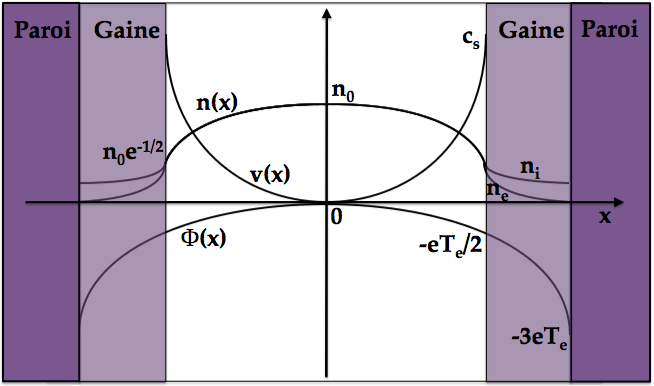
\includegraphics[width=0.7\textwidth]{figures/1-sheathprofiles.png}{\caption{Profils
des densités électronique et ionique,
du potentiel et de la vitesse ionique à
la transition plasma-gaine. La taille
de la gaine est ici exagérée.}\label{1-profilesgaine}}
\end{figure}

$\Lambda$ est le potentiel correspondant à une égalité stricte des flux au
niveau de la gaine. Cependant, il ne définit qu'une position
d'équilibre autour de laquelle le potentiel s'ajuste constamment pour
équilibrer les flux à travers la circulation des courants de gaine :

\begin{equation}
	j_{s}=en_{s}v_{i}\left(1-e^{\Lambda-(\Phi_{s}-\Phi_\text{w})/T_{e}}\right)
\end{equation}

Il est aussi possible de quantifier l'énergie perdue à la paroi par les
électrons. En admettant que les électrons ne transfèrent que de l'énergie
cinétique à la paroi quand ils sont perdus, le flux d'énergie s'écrit :

\begin{equation}
	\Gamma_\varepsilon^\text{w}=n_ev_{e}^\text{w}\varepsilon_e^\text{w}
\end{equation}

où $\varepsilon_e^\text{w}$ représente l'énergie moyenne perdue par
électron, qui peut être calculée directement en moyennant là aussi sur une
demi-maxwellienne :

\begin{equation}
	\varepsilon_e^\text{w}=\frac{1}{\sqrt{2\pi}v_{{T}_e}v_{e}^\text{w}}\int_0^\infty
	\frac{m_e}{2e}\left(v^2+2v_{{T}_e}^2\right)v\exp\left(-v^2/2v_{{T}_e}^2\right)dv
	=2T_e
\end{equation}

Pour obtenir l'énergie moyenne totale $\varepsilon_e^s$ perdu par les électrons
en entrée de gaine, il faut ajouter le potentiel de gaine à
$\varepsilon_e^\text{w}$ afin de prendre en compte l'énergie transférée aux
ions dans la chute de potentiel :

\begin{equation}
	\varepsilon_e^s=2T_e+e(\Phi_s-\Phi_\text{w})
\end{equation}

\subsubsection{Gaine dans les plasmas multi-espèces}
Le critère de Bohm pour un plasma multi-espèces a été dérivé par
Riemann~\parencite{Riemann95} ; il prend la forme :

\begin{equation}
\label{1-BohmMulti}
1\geq\sum_i{\frac{n_ic_{si}^2}{n_eu_i^2}}
\end{equation}

avec $c_{si}$ la vitesse de Bohm de l'espèce $i$.
L'inégalité \eqref{1-BohmMulti} a plusieurs solutions car le critère ne
précise pas comment les vitesses sont distribuées sur les différentes espèces.
Cependant, la seule théorie
qui autorise une solution stationnaire du plasma correspond à la situation
où chaque espèce possède sa
propre vitesse de Bohm en entrée de gaine $c_{si}$~\parencite{Allen} :

\begin{equation}
\label{1-BohmSpeed1}
v_i=c_{si}=\sqrt{T_e/m_i}
\end{equation}

Franklin montre de plus que dans le cas d'une ionisation uniforme dans l'espace,
tous les groupes d'ions atteignent leur propre vitesse de Bohm~\parencite{Franklin}. Cependant
cette théorie est controversée et discutable, certaines expérimentations
récentes la contredisant même\footnote{
L'inégalité \eqref{1-BohmSpeed1} est aussi vérifiée quand les ions ont tous la
même vitesse, sorte de vitesse de Bohm du système :
\begin{equation}
\label{1-BohmSpeed2}
v_i=c_s=\sqrt{\sum_i\frac{n_i}{n_e}c_{si}^2}
\end{equation}
Le travaux de Baalrud~\parencite{Baalrud} montrent que dans un plasma constitué
de deux espèces d'ions, la vitesse relative des espèces en entrée de gaine ne
peut pas dépasser une valeur critique $\Delta v_c=v_1-v_2$, $\Delta
v_c\rightarrow\,$0 dans la limite $T_i\rightarrow\,$0. D'autres travaux appuient
cette théorie en apportant des preuves expérimentales allant dans le sens de
cette vitesse de Bohm mixte, comme par exemple ceux de Severn et
al.~\parencite{Severn} qui montrent que, dans le cas d'un plasma argon-helium
de concentration équivalente, les ions d'argon se déplacent 75\% plus
rapidement que leur vitesse de Bohm particulière.}.
 
\subsubsection{Gaine dans les plasmas magnétisés}
La situation dans le cas d'un champ magnétique normal à la paroi est
identique au cas non-magnétisé. Quand les ions sont magnétisés, la théorie peut
de plus être étendue à une incidence $\alpha_\text{inc}$ non-rasante des lignes de champ (voir la
figure~\ref{1-sheathPerp}) où une prégaine magnétique de quelques rayons de
Larmor accélère les ions jusqu'à la vitesse de Bohm via une déflexion
imposée à la trajectoire des particules. Le critère de Bohm est alors légèrement corrigé pour tenir compte du transport
transverse lié aux dérives \cite{Stangeby} :

\begin{equation}
	v_{i_{\para}}\geq
	c_{s}-\frac{v_{i_{\perp}}}{\tan{\alpha_\text{inc}}}
\end{equation}
 
 $v_{i_{\para}}$ et $v_{i_{\perp}}$ désignant respectivement les composantes
 parallèle et perpendiculaires au champ magnétique de la vitesse ionique. La valeur critique
 de la vitesse parallèle est donc diminuée en fonction de l'importance de la
 vitesse des dérives.
 
 \begin{figure}[htbp]
\centering
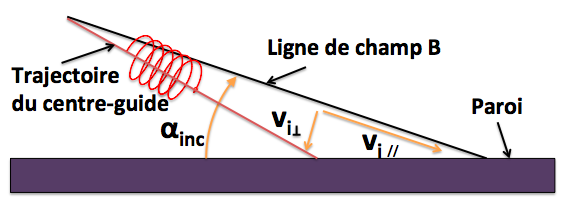
\includegraphics[width=0.7\textwidth]{figures/1-sheathPerp.png}{\caption{Cas
de lignes de champ interceptant la paroi avec une
inclinaison $\alpha_\text{inc}$.}\label{1-sheathPerp}}
\end{figure}
 
 Les cas d'un
 plasma où seuls les électrons sont magnétisés et d'une gaine totalement
 parallèle au champ magnétique s'avèrent plus complexes et ne sont pas
 clairement définis dans la littérature. Comme dans les sources
 $\lambda_D/\rho_L\ll 1$, nous supposerons que les ions
 doivent au moins atteindre la vitesse de Bohm à la sortie du plasma quasineutre.

\section{Fonction de distribution et théorie fluide}
\label{Maxwell-Boltzmann}

Le plasma est un système dynamique complexe dont l'évolution au cours du temps
peut être suivie de différentes façons. La description la plus complète utilise
une approche statistique dans laquelle chaque espèce $\alpha$ est caractérisée
par une fonction de distribution $f_\alpha(\mathbf{r},\mathbf{v},t)$
représentant le nombre moyen de particules occupant un volume infinitésimal
de l'espace des phases à un instant $t$. Son évolution est alors décrite à
travers l'équation de Boltzmann.

On peut aussi opter pour une description fluide macroscopique du plasma.
Une espèce sera alors
caractérisée par un ensemble de paramètres macroscopiques, calculés à
partir des moments de la fonction de distribution. Les plus importants -
la densité $n_\alpha$, la vitesse fluide $\mathbf u_\alpha$ et la température
$T_\alpha$ - ont des interprétations physiques immédiates et sont souvent mesurables
expérimentalement. L'évolution de ces quantités est ensuite décrite par les
équations fluides, obtenues en prenant les moments correspondants de l'équation de Boltzmann.

\subsection{L'équation de Boltzmann}
Le nombre de particules dans un plasma étant généralement élevé, il est
approprié de les représenter en fonction de chaque
espèce\footnote{La fonction de
distribution peut aussi servir à suivre les différents états quantiques des
ions, des atomes et des molécules (rotationnel, vibrationnel, électronique).}
d'une manière statistique par une fonction de
distribution $f_\alpha\text{d}\puissance{3}\mathbf r\text{d}\puissance{3}\mathbf
v$ dénombrant le nombre moyen de particules présentes à un instant $t$ dans un
volume de l'espace des phases $\text{d}\puissance{3}\mathbf r\text{d}\puissance{3}\mathbf v$.
L'évolution de cette fonction de distribution sous l'influence des forces
extérieures et des collisions est alors décrite par l'équation cinétique de
Boltzmann :

\begin{equation}
\label{1-BoltzmannEquation}
\partial_tf_\alpha+\mathbf{v}_\alpha\cdot\vec\nabla_\mathbf{r}f_\alpha+
\frac{\mathbf{F}}{m_\alpha}\cdot\vec\nabla_{\mathbf{v}}f_\alpha
=C[f_\alpha]
\end{equation}

où $\vec\nabla$ est l'opérateur gradient appliqué à l'espace des positions ou
des vitesses, et $\mathbf{F}$ la somme des forces extérieures, qui se résument
souvent aux forces électromagnétiques. Lors de collisions, les particules peuvent changer de
trajectoire, et ainsi se déplacer instantanément dans des régions éloignées de leur espace des
phases (ou encore totalement disparaître lors de collisions inélastiques).
L'opérateur de collisions $C[f_\alpha]$, qui doit représenter l'intégralité de
ces effets discrets, mesure le taux auquel les particules sont transférées d'un
volume de l'espace des phases à un autre.

 L'équation de Boltzmann permet de
suivre parfaitement l'évolution de chacune des espèces du plasma et elle est
même parfois incontournable pour décrire avec exactitude les interactions
ondes-particules ou celles impliquant des particules rapides. 

Cependant, du fait de ses 6 dimensions et de la complexité de
l'opérateur de collisions $C[f]$, \eqref{1-BoltzmannEquation} est très
lourde à résoudre numériquement et les méthodes utilisées
s'appuient sur de nombreuses approximations de la fonction de
distribution~\parencite{HagelaarHDR}. Par exemple, pour réduire le problème, on
peut approximer $f_\alpha$ dans l'espace des vitesses en supposant une
distribution ayant déjà une certaine forme et pouvant être caractérisée par une
certaine largeur. L'intégration de l'équation de Boltzmann dans l'espace des
vitesses permet alors de ne garder que les dimensions spatiales et temporelle
du système : c'est l'approche fluide.

\subsection{Les quantités fluides}
L'approche fluide consiste à décrire le comportement des particules de chaque
espèce en terme de quantités macroscopiques moyennes telles que la densité
$n$, la vitesse moyenne $\mathbf u$ et la température $T$.
Ces quantités sont définies par les moments en vitesse des fonctions de
distributions.
Pour une espèce $\alpha$ le moment en vitesse d'ordre $k$ est un tenseur d'ordre
$k$ :

\begin{equation}
\mathbf M^{(k)}_\alpha(\mathbf
r,t)=\int_{\mathbf v}\mathbf{v}^k f_\alpha(\mathbf r,\mathbf v,t)
\,\text{d}\puissance{3}\mathbf{v}
\end{equation}

Les trois premiers moments $\mathbf M^{(0)}$, $\mathbf M^{(1)}$ et $\mathbf
M^{(2)}$ ont chacun un nom et une interprétation physique simple. La densité
$n_\alpha$, qui mesure le nombre de particules de l'espèce $\alpha$ dans un
petit volume, et le flux de particules $\boldsymbol{\Gamma}_\alpha$, qui
s'exprime en fonction de la vitesse fluide $\mathbf u_\alpha$, sont
donnés par :

\begin{equation}
n_\alpha(\mathbf
r,t)=\int_{\mathbf v} f_\alpha(\mathbf r,\mathbf v,t)
\,\text{d}\puissance{3}\mathbf{v}
\end{equation}

\begin{equation}
\boldsymbol{\Gamma}_\alpha(\mathbf
r,t)=n_\alpha\mathbf u_\alpha=\int_{\mathbf v} \mathbf v f_\alpha(\mathbf
r,\mathbf v,t) \,\text{d}\puissance{3}\mathbf{v}
\end{equation}

Le moment d'ordre deux (le tenseur de pression) est mesuré dans le repère au
repos du fluide en introduisant la vitesse relative $\mathbf w=\mathbf
v-\mathbf u_\alpha$ : 

\begin{equation}
\mathbf P_\alpha(\mathbf
r,t)=m_\alpha\int_{\mathbf v} \left(\mathbf
v-\mathbf u_\alpha\right)\left(\mathbf
v-\mathbf u_\alpha\right)
f_\alpha(\mathbf r,\mathbf v,t) \,\text{d}\puissance{3}\mathbf{v}
\end{equation}

le tenseur de pression mesure l'écart quadratique entre la vitesse moyenne des
particules et la vitesse fluide. On introduit ensuite la
pression scalaire $p_\alpha$ et le tenseur de viscosité
$\boldsymbol{\Pi}_\alpha$, tels que:

\begin{equation}
\label{1-tenseurPression}
\mathbf P_\alpha=p_\alpha\,\mathbf I + \boldsymbol{\pi}_\alpha
\end{equation}

avec $\mathbf I$ la matrice identité. Par analogie avec la théorie fluide
conventionnelle, on s'attend à ce que les termes diagonaux soient dominants
quand l'espèce est à l'équilibre thermique. La trace du tenseur
$\mathbf P_\alpha$ quantifie ainsi la densité d'énergie cinétique
interne de l'espèce et peut se réécrire en définissant la température partielle 
$T_\alpha$ mesurée en unité d'énergie :

\begin{equation}
\frac{3}{2}p_\alpha=\frac{3}{2}n_\alpha
T_\alpha=\frac{m_\alpha}{2}\int_{\mathbf v} w\puissance{2} f_\alpha(\mathbf
r,\mathbf v,t) \,\text{d}\puissance{3}\mathbf{v}
\end{equation}

En montant en ordre, les moments apportent de plus en plus de détails sur la
fonction de distribution, donnant théoriquement une description du plasma
strictement équivalente à la description statistique. Dans les fluides
collisionnels (et plus précisément quand les auto-collisions sont suffisamment
nombreuses), il ne suffit généralement que de la densité $n_\alpha$, de la
vitesse $\mathbf{u}_\alpha$ et de la température $T_\alpha$ pour caractériser l'ensemble des particules d'une espèce, les fonctions de distribution
prenant la forme de maxwelliennes locales\footnote{Il suffit de deux vitesses
pour caractériser une maxwellienne, la vitesse moyenne $\left<v\right>$ et la vitesse quadratique moyenne $\sqrt{\left<v\puissance{2}\right>}$ :
$$
	\left<v\right>=\sqrt{\frac{8T}{\pi m}} \;\;\;\;\text{et}\;\;\;\; 
	\left<v\puissance{2}\right>=\frac{3T}{m}
$$ 
Les moments de la fonction de distribution se calculent ainsi facilement.}:
\begin{equation}
\label{1-MaxwellDistribution}
	f_\alpha\simeq n_\alpha
	\left(\frac{m_\alpha}{2\pi
	T_\alpha}\right)\puissance{3/2}\exp\left(\frac{-m_\alpha \left(\mathbf
	v_\alpha-\mathbf u_\alpha\right)\puissance{2}}{2T_\alpha}\right)
\end{equation}

Pour une espèce dont la fonction de distribution n'est à priori pas
maxwellienne, on réalise une opération de fermeture du système d'équations, qui,
à l'ordre $k$, consiste à approximer ou exprimer les moments d'ordre $k$+1
en fonction des moments d'ordre inférieur et de leur gradient.

\subsection{Les équations de conservation}

À chaque quantité macroscopique est adjointe une équation traduisant sa
conservation. Ces équations de conservation, aussi appelées équations fluides,
sont obtenues en prenant les moments correspondants de l'équation de Boltzmann.

\subsubsection{Conservation de la matière}
L'équation de conservation de la matière contrôle
l'évolution de la densité. On l'obtient en intégrant
l'équation de Boltzmann (\eqref{1-BoltzmannEquation}) sur l'espace des
vitesses~:

\begin{equation}
\label{1-eqContinuite}
	\partial_tn_\alpha+
	\nabla\cdot\left(n_\alpha\mathbf{u_\alpha}\right)=\mathcal{S}_\alpha
\end{equation}

avec $n_\alpha$ la densité de l'espèce, $\mathbf{u_\alpha}$ la vitesse
fluide et $\mathcal{S}_\alpha$ un terme source se mesurant en
nombre de particules par unité de temps et de volume. Dans
les plasmas froids, ce terme rend compte
du nombre de particules ionisées ou perdues lors de collisions inélastiques ;
issu de l'intégration de l'opérateur de collision, il regroupe
l'ensemble des interactions collisionnelles et chimiques :

\begin{equation}
	\mathcal{S}_\alpha=\sum_{j} N_j n_{\alpha}n_{s}
	k_j
\end{equation} 

où $j$ dénote une interaction, $N_j$ est le nombre de particules
créées lors d'une collision (négatif en cas de destruction), $n_\alpha$ et $n_s$
la densité des espèces en collision et $k_{j}=\left<\sigma_{j}
v_r\right>$ le coefficient de collision/réaction associé
(cf.\S~\ref{1-Collisions}), avec $v_r=(\mathbf u_s-\mathbf u_\alpha)$ la
vitesse relative des deux fluides. Le terme source peut ensuite se décomposer en une
partie positive liée à la création par ionisation et à une partie négative due à la recombinaison :

\begin{equation}
	\mathcal{S}_\alpha=\mathcal{S}_\alpha^++\mathcal{S}_\alpha^-\sim
	n_{\alpha}\nu_\alpha^\text{iz}-n_{\alpha}\nu_\alpha^\text{re}
\end{equation} 


\subsubsection{Conservation de la quantité de mouvement}
L'équation de conservation de la quantité de mouvement peut être considérée
comme le moment d'ordre un en vitesse de l'équation de Boltzmann. En multipliant
\eqref{1-BoltzmannEquation} par $\mathbf v$ puis en intégrant sur l'espace des
vitesses, on obtient :

\begin{equation}
\label{1-eqQuantiteMouvement}
\partial_t m_\alpha n_\alpha \mathbf{u}_\alpha + 
\nabla\cdot\left(m_\alpha n_\alpha
\mathbf{u}_\alpha\mathbf{u}_\alpha+\mathbf{P_\alpha}\right)=q_\alpha
n_\alpha\left(\mathbf E+\mathbf u_\alpha\times\mathbf B\right)
+\mathbf{R_\alpha}
\end{equation}

avec $\mathbf{P_\alpha}$ le tenseur de pression, $\mathbf{E}$ et $\mathbf{B}$
les forces électromagnétiques et $\mathbf{R_\alpha}$ un terme de
friction traduisant la perte et l'échange de quantité de mouvement dans les
collisions. En toute généralité, on peut écrire ce transfert de quantité de
mouvement pour chaque espèce $\alpha$ comme une somme de deux composantes :

\begin{equation}
\mathbf{R_\alpha}=\mathbf{R}_{\alpha}^{(\mathbf
u)}+\mathbf{R}_{\alpha}^{(T)}
\end{equation}

Le terme
$\mathbf{R}_{\alpha}^{(T)}$ est connu sous le nom de force thermique et
émerge de la dépendance en vitesse des fréquences de collision (il est
généralement négligé dans les modèles de plasmas froids).
Le terme $\mathbf{R}_{\alpha}^{(\mathbf u)}$ est une force de frottement
proportionnelle à la vitesse relative des espèces en collision :

\begin{equation}
\mathbf{R}_{\alpha}^{(\mathbf
u)}=n_\alpha\sum_{s\neq\alpha}\frac{m_\alpha m_s}{m_\alpha+m_s}
n_sk^\text{m}_{\alpha s} \left(\mathbf u_s-\mathbf u_\alpha\right)
\end{equation}

où $k^\text{m}_{\alpha s}=\left<\sigma^\text{m}_{\alpha s}v_r\right>$ est un
taux efficace de transfert de quantité de mouvement.
Dans le cas de plasmas fortement ionisés ne contenant qu'une seule espèce et où
les collisions coulombiennes sont dominantes, $\mathbf{R_\alpha}$ s'exprime à
travers la fermeture de Braginsky en fonction du courant $\mathbf
j=en\left(\mathbf u_i-\mathbf u_e\right)$ et du gradient de température
électronique $\nabla T_e$~\parencite{Braginsky}. Dans le cadre des plasmas
froids, c'est les collisions avec le gaz au repos qui sont dominantes et le
terme de friction se réécrit :

\begin{equation}
\label{1-forceFriction}
\mathbf{R_{\alpha}}=\mathbf{R_{\alpha}^{(\mathbf
u)}}=m_\alpha n_\alpha\mathbf u_\alpha\sum_{s\neq\alpha}\frac{m_s}{m_\alpha+m_s}
n_sk^\text{m}_{\alpha s} = m_\alpha n_\alpha \nu_\alpha \mathbf u_\alpha
\end{equation}

En remplaçant les expressions du
tenseur de pression (\eqref{1-tenseurPression}) et du terme de friction (\eqref{1-forceFriction}) dans
\eqref{1-eqQuantiteMouvement}, puis en la combinant avec l'équation de
continuité (\eqref{1-eqContinuite}), on obtient l'équation qui contrôle
l'évolution de la vitesse :

\begin{equation}
\label{1-eqMouvement}
\partial_t \mathbf{u}_\alpha + (\mathbf{u}_\alpha\cdot\nabla)\mathbf{u}_\alpha
+\left(\nu_\alpha+\nu_\alpha^\text{iz}\right) \mathbf
u_\alpha=\frac{q_\alpha}{m_\alpha}\left(\mathbf E+\mathbf u_\alpha\times \mathbf
B\right) -\frac{\nabla p_\alpha}{m_\alpha n_\alpha}
-\frac{\nabla\cdot\boldsymbol{\pi}_\alpha}{m_\alpha n_\alpha}
\end{equation}

où $\nu_\alpha^{\text{iz}}=\mathcal{S}^+_\alpha/n_\alpha$ provient de la
substitution de l'équation de continuité et caractérise la quantité de mouvement
perdue avec l'ionisation : la création de particules sans
vitesse initiale apparaît pour le fluide comme une perte effective de quantité
de mouvement, entraînant une force nette proportionnelle à la vitesse
du fluide, $\mathbf F=\mathbf{u_\alpha}
\nu_\alpha^{\text{iz}}$. Bien que l'on ne
réalise pas souvent l'importance de ce phénomène, il est crucial pour décrire
correctement l'évolution des espèces ioniques dans un plasma
froid\footnote{Rigoureusement, cette expression n'est valide que tant que les
particules sont perdues à la vitesse moyenne $\mathbf u_\alpha$, auquel cas
$\mathcal{S}^-$ n'intervient pas.
Si l'on considère que les particules sont perdues avec une vitesse de
préférence différente de $\mathbf u_\alpha$, il faut inclure le terme
correspondant de gain/perte de quantité de mouvement.}.

\subsubsection{Conservation de l'énergie}
\label{1-ConservationEnergie}
Le deuxième moment de l'équation de Boltzmann donne une équation tensorielle
dont la contraction garantit la conservation de l'énergie moyenne du système.
L'équation de conservation de
l'énergie, qui s'obtient également en multipliant \eqref{1-BoltzmannEquation}
par $m_\alpha {u}_\alpha^2/2$, s'écrit :

\begin{equation}
\label{1-eqEnergie}
\partial_t n_\alpha\varepsilon_\alpha+
\nabla\cdot\left(n_\alpha\varepsilon_\alpha\mathbf{u}_\alpha+\mathbf
P_\alpha\cdot\mathbf{u}_\alpha + \mathbf q_\alpha\right) =q_\alpha
n_\alpha\mathbf E\cdot
\mathbf{u}_\alpha+\Pi_\alpha
\end{equation}

où $\varepsilon_\alpha$ est l'énergie
moyenne du fluide, qui se compose de l'énergie thermique et de l'énergie dirigée
$\,\mathcal{U}_{\alpha}=m_\alpha u_\alpha^2/2$ :

\begin{equation}
\varepsilon_\alpha=\frac{3}{2}T_\alpha+\mathcal{U}_\alpha
\end{equation}

 L'équation fait intervenir le
troisième moment de la fonction de distribution $\mathbf q_\alpha$, qui
représente le flux de chaleur (d'énergie chaotique), i.e. le flux d'énergie dans
le repère au repos du fluide :

\begin{equation}
	\mathbf q_\alpha=\frac{1}{2}m_\alpha
	n_\alpha\left<w^2\mathbf w\right>
\end{equation} 

Enfin, $\Pi_\alpha$ est la production \emph{totale}\footnote{Dans de
nombreux ouvrages, le terme de chauffage collisionnel est décomposé en un terme de chauffage dirigé et un terme mesurant
le chauffage dans le repère au repos ${W}_\alpha$:
$$\Pi_\alpha=\int_{\mathbf v}\frac{m_\alpha}{2}v_\alpha^2C_\alpha
d\mathbf v=\int_{\mathbf v}\frac{m_\alpha}{2}(u_\alpha+w_\alpha)^2C_\alpha d\mathbf
v\sim{W}_\alpha+\mathbf u_\alpha\cdot\mathbf R_\alpha $$ Après le
travail algébrique sur les équations pour obtenir la conservation de l'énergie
thermique (qui annule le terme $q_\alpha n_\alpha\mathbf E\cdot\mathbf
u_\alpha$), le terme $\mathbf u_\alpha\cdot\mathbf R_\alpha$ disparaît pour ne laisser que le terme ${W}_\alpha$. 

En pratique, le
${W}_\alpha$ est difficile à évaluer, et les expériences nous donnent
plutôt accès à la variation totale de l'énergie.
Dans ce manuscrit, nous
considérerons la perte d'énergie totale dans les équations ; le terme de
chauffage par friction (i.e.
l'effet Joule) est donc toujours présent après la substitution dans l'équation d'énergie.} de chaleur lors de collisions et de
réactions chimiques.
Pour les électrons, cette puissance collisionnelle est généralement négative et peut s'exprimer en terme de taux:

\begin{equation}
	\Pi_e=\int_{\mathbf
	v}\frac{m_\alpha}{2}v^2C_\alpha \text{d}^3\mathbf
	v=-en_e\sum_{j}\left(E_jn_sk_{j}\right)-en_e\sum_{s}\left(\frac{2m_e}{m_s}n_sk^m_{es}\varepsilon_e\right)=-en_en_gk_e^\varepsilon
\end{equation}

avec $\Theta_e^\varepsilon$ un taux de puissance moyenne perdue par électron. 
Le premier terme donne la perte d'énergie inélastique sommée sur l'ensemble
des processus d'excitation et d'ionisation $j$, avec $E_j$ l'énergie de seuil de
la réaction. Le second terme représente la perte d'énergie dans les collisions
élastiques. Dans un cas simple, en ne considérant que l'ionisation et les
collisions élastiques avec le gaz, l'expression de $\Pi_e$
se simplifie :

\begin{equation}
	\Pi_e\approx-en_en_g\left(E_\text{iz}k_\text{iz}+\frac{2m_e}{m_g}k^m_e\varepsilon_e\right)
\end{equation}



On peut
maintenant soustraire la contribution de l'énergie dirigée
$\mathcal{U}_{\alpha}$ de \eqref{1-eqEnergie} en utilisant le produit scalaire
de l'équation de conservation de la quantité de mouvement
(\eqref{1-eqQuantiteMouvement}) et de la vitesse fluide pour obtenir une
équation de conservation sur l'énergie interne (thermique) d'une espèce :

\begin{equation}
\label{1-eqEnergieInterne}
\frac{3}{2}\partial_t p_\alpha + 
\nabla\cdot\left(\frac{3}{2}p_\alpha
\mathbf{u}_\alpha+\mathbf q_\alpha\right)+p_\alpha\nabla\cdot\mathbf u_\alpha
+\boldsymbol{\pi}_{\alpha j k}\frac{\partial u_{\alpha j}}{\partial{x_k}} =
{\Pi_\alpha}+(2n_\alpha\nu_\alpha+\mathcal{S}_\alpha)\,\mathcal{U}_\alpha
\end{equation}

Dans cette équation, $p_\alpha\nabla\cdot\mathbf u_\alpha$ représente la
puissance produite par la pression partielle qui résulte du
refroidissement/chauffage lié à la compression ou à l'expansion d'un volume de
plasma. Le terme $\boldsymbol{\pi}_{\alpha j k}\partial u_{\alpha
j}/\partial{x_k}$, qui décrit le chauffage visqueux, est souvent négligé
devant le terme $(2n_\alpha\nu_\alpha+\mathcal{S}_\alpha)\,\mathcal{U}_\alpha$, 
qui apparaît distinctement comme une production de chaleur
à travers les collisions, et comprend notamment le chauffage ohmique. Ce
 terme est primordial pour capturer correctement le comportement de la
température électronique dans les plasmas froids.

En utilisant l'équation de
continuité pour réduire l'équation d'énergie (\eqref{1-eqEnergieInterne}), on
obtient une équation d'évolution pour la température de l'espèce :

\begin{equation}
\label{1-eqTemperature}
\frac{3}{2}n_\alpha\frac{\text{d}T_\alpha}{\text{dt}}+\nabla\cdot\mathbf
q_\alpha + n_\alpha T_\alpha\nabla\cdot\mathbf u_\alpha +
\frac{3}{2}\mathcal{S}_\alpha T_\alpha =
{\Pi_\alpha}+(2n_\alpha\nu_\alpha+\mathcal{S}_\alpha)\,\mathcal{U}_\alpha
\end{equation}

avec $\text{d}/\text{dt}=\partial_t+\mathbf u\cdot\nabla$ la notation de la
dérivée convective. En substituant enfin le terme de compression
$p_\alpha\nabla\cdot\mathbf u_\alpha$ pour faire disparaître la divergence de la
vitesse, \eqref{1-eqTemperature} se réécrit :

\begin{equation}
\label{1-eqTemperature2}
\frac{3}{2}n_\alpha\frac{\text{d}T_\alpha}{\text{dt}}+\nabla\cdot\mathbf
q_\alpha + \frac{5}{2}\mathcal{S}_\alpha T_\alpha =
T_\alpha\frac{\text{d}n_\alpha}{\text{dt}}+
{\Pi_\alpha}+(2n_\alpha\nu_\alpha+\mathcal{S}_\alpha)\,\mathcal{U}_\alpha
\end{equation}

Dans notre étude des plasmas froids magnétisés, la température ionique $T_i$
est très proche de celle des neutres et il n'est pas nécessaire de décrire
son évolution. $T_e$ en revanche joue un rôle primordial dans le comportement
du plasma car directement responsable de l'ionisation du gaz et donc du
transport collisionnel généré. 

Le plus souvent, la fermeture du système d'équations fluides se réalise sur le
flux de chaleur $\mathbf q_e$, qui s'exprime alors en fonction d'une
conductivité thermique et du gradient de température. Dans les conditions des plasmas froids
basse-pression magnétisés, le flux de chaleur porté par les électrons est
cependant très sensible au champ magnétique et tend à influencer de façon
notable le comportement de $T_e$ ; il doit donc être décrit avec attention à
travers une équation spécifique.

\subsubsection{Conservation de la chaleur électronique}

Les équations \eqref{1-eqEnergieInterne}-\eqref{1-eqTemperature2} font
intervenir des moments d'ordre trois, les composantes du vecteur de flux de
chaleur $\mathbf q_\alpha$ dont les expressions sont assez similaires et se
dérivent de la même façon que celles du flux de particules. Quand les électrons
sont suffisamment collisionnels et que l'énergie dirigée est inférieure à
l'énergie thermique ($m_eu_e^2/2\ll T_e$), l'équation pour le flux de chaleur
électronique prend la forme~\parencite{Golant} :

\begin{equation}
\label{1-eqFluxChaleur}
\partial_t\mathbf
q_e+\frac{5}{2}\frac{n_e
T_e}{m_e}\nabla T_e+\frac{e}{m_e} \mathbf
q_e\times\mathbf B=\left[\frac{\delta\mathbf q_e}{\delta t}\right]_\text{coll}
\end{equation}

Dans le deuxième terme de \eqref{1-eqFluxChaleur}, le
gradient de température, moteur du flux de chaleur, est multiplié par une
conductivité thermique du plasma $5n_eT_e/2m_e$, approximation classique pour
refermer le système~\parencite{bittencourt}. Le terme de collision
$\delta\mathbf q_e/\delta t$ peut enfin s'exprimer en fonction d'une fréquence
caractéristique de diffusion de chaleur par collision $\nu_{e}^\varepsilon$.
\eqref{1-eqFluxChaleur} se réécrit :

\begin{equation}
\label{1-eqFluxChaleur2}
\partial_t\mathbf
q_e+\frac{5}{2}\frac{n_e
T_e}{m_\alpha}\nabla T_e+\frac{e}{m_e} \mathbf q_e\times\mathbf
B=-\nu_{e}^\varepsilon\mathbf q_e
\end{equation}
La fréquence $\nu_e^\varepsilon$ regroupe alors l'ensemble des collisions, y
compris les auto-collisions :
\begin{equation}
\nu_e^\varepsilon=\nu_{en}^\varepsilon+\nu_{ei}^\varepsilon+\nu_{ee}^\varepsilon\footnote{La fréquence de diffusion de chaleur lors des
collisions avec le gaz dominantes et isotropes, cette fréquence est à peu près
égale à la fréquence de transfert de quantité de mouvement $\nu_{en}^\varepsilon\approx\nu_{en}^m$ }
\end{equation} Le système \{\textup{\ref{1-eqContinuite},
\ref{1-eqQuantiteMouvement}, \ref{1-eqEnergieInterne}, \ref{1-eqFluxChaleur}}\}
forme une suite d'équations de conservation décrivant le comportement et
l'évolution des espèces dans le plasma.
Ces équations sont rigoureusement valides pour des échelles de temps et d'espace
grandes devant les échelles caractéristiques collisionnelles :

\begin{equation}
\omega\ll \nu_{\alpha}
\;\;\;\;\text{et}\;\;\;\;l\gg\lambda_\alpha=\frac{c_s}{\nu_\alpha}
\end{equation}

Il peut sembler qu'une description fluide d'un plasma soit fortement limitée par
cette hypothèse. Cependant, dans un plasma, l'interaction globale des
particules chargées change ces considérations.
Les électrons, confinés par le potentiel de gaine et ralentis par leur
couplage avec les ions, peuvent se maxwelliser même sans collision. 

Il arrive alors, bien qu'elle ne soit pas rigoureusement justifiée,
que l'application de la théorie fluide en
dehors du domaine de validité des équations donne des résultats intéressants,
tant au niveau qualitatif que quantitatif,
pour toute une variété de configurations, validant a posteriori le choix de son
utilisation.
Même si elles ne peuvent capter l'ensemble de la
physique cinétique et les interactions ondes-particules, les équations fluides
contiennent déjà énormément de physique et restent suffisantes dans de
nombreuses situations.

La théorie fluide, en supposant une cohésion macroscopique de l'ensemble des
particules, fournit une description de base pour étudier les phénomènes de
transport dans les plasmas. À partir de ce formalisme, la plupart des modèles
sont construits en simplifiant les équations pour ne retenir que
les caractéristiques et processus essentiels du système à étudier. 

\end{refsection}

